\documentclass[conference]{IEEEtran}
\IEEEoverridecommandlockouts
% The preceding line is only needed to identify funding in the first footnote. If that is unneeded, please comment it out.
\usepackage{cite}
\usepackage{amsmath,amssymb,amsfonts}
\usepackage{algorithmic}
\usepackage{graphicx}
\usepackage{textcomp}
\usepackage{xcolor}
\usepackage{booktabs}
\usepackage{multirow}
\usepackage{array}
\usepackage{url}
\def\BibTeX{{\rm B\kern-.05em{\sc i\kern-.025em b}\kern-.08em
    T\kern-.1667em\lower.7ex\hbox{E}\kern-.125emX}}

\begin{document}

\title{The Visual Instruction Following Evaluation Benchmark (VIF-Eval): A Comprehensive Framework for Evaluating Compositional and Editorial Image Generation}

\author{\IEEEauthorblockN{[Your Name/Team]}
\IEEEauthorblockA{\textit{[Your Institution]}\\
[Your City, Country]\\
[email@example.com]}
}

\maketitle

\begin{abstract}
This paper introduces the Visual Instruction Following Evaluation Benchmark (VIF-Eval), a comprehensive framework for assessing the capabilities of generative visual models in real-world scenarios involving complex image creation, editing, and compositional reasoning. Unlike traditional text-to-image benchmarks that focus on simple prompt adherence, VIF-Eval evaluates models across multiple dimensions including complex compositional reasoning, text rendering accuracy, constraint satisfaction problems (CSP), character consistency, and sketch-to-render translation. We evaluate three state-of-the-art models—GPT Image 1, DALL-E 3, and Gemini 2.5 Flash Image (Nano Banana)—across 47 diverse prompts with 167+ constraints. Our results reveal significant performance variations across constraint types, with models achieving 54.7--58.1\% overall pass rates on standard constraints but struggling with text rendering (13.0\% pass rate) and complex compositional tasks. The benchmark provides actionable insights for improving generative AI systems and establishes a foundation for future research in visual instruction following.
\end{abstract}

\begin{IEEEkeywords}
Image Generation, Visual AI, Benchmark Evaluation, Compositional Reasoning, Text-to-Image Models
\end{IEEEkeywords}

\section{Introduction}

\subsection{Background}
Generative visual models have achieved remarkable progress in recent years, enabling high-quality image synthesis from text prompts. Models like DALL-E 3, Midjourney, Stable Diffusion, and GPT Image 1 have demonstrated impressive capabilities in creating photorealistic and artistic images. However, as these models are increasingly deployed in real-world applications—including e-commerce, advertising, design, and creative industries—there is a growing need to evaluate their performance beyond simple aesthetic quality.

\subsection{Motivation and Industry Relevance}
Real-world visual generation tasks often require: (1) \textit{Complex Compositional Reasoning}: Correctly placing multiple objects with specific attributes and spatial relationships; (2) \textit{Accurate Text Rendering}: Generating legible text within images for posters, labels, and advertisements; (3) \textit{Constraint Satisfaction}: Following mathematical and logical constraints (e.g., nutrition labels, data tables); (4) \textit{Consistency}: Maintaining character appearance and style across multiple scenes; and (5) \textit{Precision Editing}: Modifying specific image regions while preserving context.

Current benchmarks primarily focus on prompt-image alignment using metrics like CLIP score or human preference ratings, but fail to assess these critical capabilities systematically.

\subsection{Gap Analysis}
Existing text-to-image evaluation frameworks have several limitations: (1) \textit{Limited Task Diversity}: Most benchmarks focus on single-object generation or simple scene composition; (2) \textit{Lack of Automated Precision Metrics}: Heavy reliance on human evaluation makes large-scale assessment impractical; (3) \textit{Missing Constraint Validation}: No systematic evaluation of logical, mathematical, or compositional constraints; and (4) \textit{Insufficient Real-World Scenarios}: Benchmarks often use abstract or artistic prompts rather than practical use cases.

VIF-Eval addresses these gaps by providing: a comprehensive task taxonomy covering 9 constraint types, automated evaluation metrics for each constraint type, real-world inspired prompts (nutrition labels, posters, product compositions), and systematic error analysis and failure pattern identification.

\subsection{Contributions}
This paper makes the following contributions: (1) \textit{Comprehensive Benchmark}: A new evaluation framework with 47 diverse prompts and 167+ constraints; (2) \textit{Multi-Model Evaluation}: Systematic comparison of three state-of-the-art models; (3) \textit{Automated Evaluation Pipeline}: CLIP-based, OCR-based, and computer vision metrics for objective assessment; (4) \textit{Error Analysis}: Detailed categorization of failure modes and model limitations; and (5) \textit{Open-Source Implementation}: Complete evaluation codebase and dataset for reproducibility.

\section{Methodology}

\subsection{Visual Task Taxonomy}
VIF-Eval defines a comprehensive taxonomy of visual instruction following tasks:

\subsubsection{Complex Prompt Adherence}
\textit{Count Constraints}: Verify correct number of objects (e.g., ``three blue mugs''). \textit{Attribute Constraints}: Verify object attributes (e.g., color, size, material). \textit{State Constraints}: Verify object states (e.g., ``tipped over'', ``empty''). \textit{Spatial Constraints}: Verify spatial relationships (e.g., ``left of'', ``above'').

\subsubsection{Text Rendering}
\textit{Poster Text}: Rendering legible text in poster designs. \textit{Label Text}: Accurate text in nutrition labels and product information. \textit{Banner Text}: Text in advertising banners and headers.

\subsubsection{Constraint Satisfaction Problems (CSP)}
\textit{Numeric Relations}: Mathematical relationships (A $<$ B, A + B = C). \textit{Sorting}: Ordered sequences (ascending, descending). \textit{Uniqueness}: All-different constraints. \textit{Range Constraints}: Value bounds (min $\leq$ x $\leq$ max). \textit{Complex Operations}: Products, ratios, differences, modulo.

\subsubsection{Style \& Character Consistency}
\textit{Character Consistency}: Same character across multiple scenes. \textit{Attribute Preservation}: Maintaining clothing, appearance, accessories.

\subsubsection{Image-to-Image Translation}
\textit{Sketch-to-Render}: Converting simple sketches to photorealistic renders. \textit{Structural Fidelity}: Preserving structural elements while enhancing detail.

\subsection{Dataset Creation}

\subsubsection{Prompt Sourcing}
Our prompt suite consists of 47 prompts across 7 categories: (1) \textit{Composition} (6 prompts): Multi-object scenes with count, attribute, state, and spatial constraints; (2) \textit{Poster Text} (6 prompts): Advertising posters requiring accurate text rendering; (3) \textit{Nutrition Labels} (6 prompts): Food labels with structured data and text; (4) \textit{CSP Demo} (13 prompts): Mathematical and logical constraint satisfaction; (5) \textit{Advanced} (6 prompts): Complex multi-constraint scenarios; (6) \textit{Character Consistency} (6 prompts): Character appearance across scenes; and (7) \textit{Sketch-to-Render} (5 prompts): Sketch translation tasks.

Prompts were designed to reflect real-world use cases (e-commerce, advertising, design), include multiple constraints per prompt for comprehensive evaluation, cover edge cases and challenging scenarios, and balance difficulty across constraint types.

\subsubsection{Data Annotation}
Each prompt is annotated with: \textit{Category}: Task category (composition, text, CSP, etc.); \textit{Constraints}: List of constraint objects with constraint type, required fields, and expected values or relationships; and \textit{Metadata}: Prompt ID, description, difficulty level.

\subsubsection{Dataset Statistics}
Total Prompts: 47. Total Constraints: 167--172 (varies by model due to special evaluators). Constraint Types: 11 distinct types. Categories: 7 categories. Average Constraints per Prompt: 3.5.

\subsection{Evaluation Metrics}

\subsubsection{Automated Metrics}
\textit{CLIP-Based Metrics}: Composition scoring using CLIP similarity for count, attribute, and state constraints; negative constraint scoring using inverse CLIP similarity for forbidden concepts; and prompt adherence using CLIP score for overall prompt-image alignment.

\textit{OCR-Based Metrics}: Text accuracy using Character Error Rate (CER) for text rendering; label parsing for field extraction accuracy in structured data; and CSP validation for numeric value extraction and constraint satisfaction.

\textit{Computer Vision Metrics}: SSIM (Structural Similarity Index) for sketch-to-render tasks; edge alignment using Intersection over Union (IoU) of edge maps; object detection using GroundingDINO for spatial relationship validation; and face recognition using InsightFace for character consistency.

\textit{Scoring Methodology}: All scores normalized to [0, 1] range with pass threshold of 0.5. Binary constraints return 1.0 (satisfied) or 0.0 (not satisfied). Continuous constraints use logistic or exponential decay functions.

\subsubsection{Constraint-Specific Metrics}
(1) \textit{Count}: Margin-based logistic scoring comparing target count to alternatives. (2) \textit{Attribute}: CLIP similarity margin between attribute and plain object. (3) \textit{Text}: Character Error Rate with exponential decay: $\exp(-3.0 \times \text{CER})$. (4) \textit{CSP}: Binary satisfaction or relative error-based scoring. (5) \textit{Spatial}: Binary validation of bounding box relationships. (6) \textit{Character Consistency}: Average of face similarity, detection consistency, and attribute consistency.

\subsubsection{Aggregation Metrics}
Pass Rate: Percentage of constraints with score $>$ 0.5. Average Score: Mean score across all constraints. Per-Type Performance: Pass rates and average scores by constraint type. Per-Category Performance: Pass rates and average scores by prompt category.

\subsection{Models Evaluated}

\subsubsection{GPT Image 1}
Provider: OpenAI. Model: gpt-image-1. Configuration: 1024$\times$1024, high quality. API: OpenAI Images API.

\subsubsection{DALL-E 3}
Provider: OpenAI. Model: dall-e-3. Configuration: 1024$\times$1024, HD quality. API: OpenAI Images API. Note: Evaluation incomplete due to API billing limits (11/47 prompts completed).

\subsubsection{Gemini 2.5 Flash Image (Nano Banana)}
Provider: Google (via OpenRouter). Model: google/gemini-2.5-flash-image. Configuration: 1024$\times$1024, high quality. API: OpenRouter API (OpenAI-compatible interface).

\section{Results}

\subsection{Overall Performance}

\begin{table}[!t]
\renewcommand{\arraystretch}{1.3}
\caption{Overall Performance Comparison}
\label{tab:overall}
\centering
\begin{tabular}{lcccc}
\toprule
Model & Prompts & Constraints & Passed & Pass Rate \\
\midrule
GPT Image 1 & 47 & 167 & 97 & 58.1\% \\
Nano Banana & 47 & 172 & 94 & 54.7\% \\
DALL-E 3 & 47 & 76 & 13 & 17.1\% \\
\bottomrule
\end{tabular}
\end{table}

Table~\ref{tab:overall} shows the overall performance comparison. GPT Image 1 achieves the highest overall pass rate (58.1\%), while Nano Banana performs comparably (54.7\%). DALL-E 3 evaluation is incomplete; partial results show 17.1\% pass rate (likely due to incomplete evaluation).

\begin{figure}[!t]
\centering
\includegraphics[width=\columnwidth]{paper_assets/figures/overall_pass_rate_comparison.png}
\caption{Overall Pass Rate Comparison Across Models}
\label{fig:overall_pass}
\end{figure}

\subsection{Performance by Constraint Type}

\begin{table*}[!t]
\renewcommand{\arraystretch}{1.2}
\caption{Performance by Constraint Type}
\label{tab:by_type}
\centering
\begin{tabular}{lccccccc}
\toprule
\multirow{2}{*}{Constraint Type} & \multicolumn{3}{c}{GPT Image 1} & \multicolumn{3}{c}{Nano Banana} & \multicolumn{1}{c}{DALL-E 3} \\
\cmidrule(lr){2-4} \cmidrule(lr){5-7} \cmidrule(lr){8-8}
 & Total & Passed & Pass Rate & Total & Passed & Pass Rate & Pass Rate \\
\midrule
Spatial & 2 & 2 & 100.0\% & 2 & 2 & 100.0\% & N/A \\
Character Consistency & 4 & 4 & 100.0\% & 4 & 4 & 100.0\% & N/A \\
CSP & 20 & 20 & 100.0\% & 20 & 19 & 95.0\% & N/A \\
Negative & 23 & 23 & 100.0\% & 24 & 24 & 100.0\% & N/A \\
State & 6 & 5 & 83.3\% & 6 & 2 & 33.3\% & 0.0\% \\
Attribute & 20 & 11 & 55.0\% & 21 & 9 & 42.9\% & 37.5\% \\
Table Slot & 42 & 20 & 47.6\% & 42 & 23 & 54.8\% & N/A \\
Count & 16 & 5 & 31.2\% & 17 & 3 & 17.6\% & 0.0\% \\
Logic & 6 & 3 & 50.0\% & 6 & 4 & 66.7\% & N/A \\
Text & 23 & 3 & 13.0\% & 25 & 3 & 12.0\% & N/A \\
Sketch-to-Render & 5 & 1 & 20.0\% & 5 & 1 & 20.0\% & N/A \\
\bottomrule
\end{tabular}
\end{table*}

Table~\ref{tab:by_type} presents detailed performance by constraint type. Models excel at spatial relationships (100\% pass rate), character consistency (100\%), and CSP constraints (95--100\%). However, they struggle significantly with text rendering (12--13\% pass rate) and counting (17--31\% pass rate).

\begin{figure*}[!t]
\centering
\includegraphics[width=0.95\textwidth]{paper_assets/figures/pass_rate_by_type_comparison.png}
\caption{Pass Rate by Constraint Type Across Models}
\label{fig:pass_by_type}
\end{figure*}

\begin{figure*}[!t]
\centering
\includegraphics[width=0.95\textwidth]{paper_assets/figures/avg_score_by_type_comparison.png}
\caption{Average Score by Constraint Type Across Models}
\label{fig:avg_score}
\end{figure*}

\subsection{Performance by Category}

\begin{table}[!t]
\renewcommand{\arraystretch}{1.3}
\caption{Performance by Category (GPT Image 1)}
\label{tab:by_category_gpt}
\centering
\begin{tabular}{lcc}
\toprule
Category & Passed/Total & Pass Rate \\
\midrule
CSP Demo & 20/20 & 100.0\% \\
Composition & 21/27 & 77.8\% \\
Advanced & 14/28 & 50.0\% \\
Nutrition Label & 30/60 & 50.0\% \\
Poster Text & 7/23 & 30.4\% \\
\bottomrule
\end{tabular}
\end{table}

\subsection{Key Insights}

\textit{Strong Performance Areas}: (1) Spatial relationships: 100\% pass rate (both models); (2) Character consistency: 100\% pass rate (both models); (3) CSP constraints: 95--100\% pass rate; and (4) Negative constraints: 100\% pass rate (avoiding forbidden concepts).

\textit{Challenging Areas}: (1) Text rendering: 12--13\% pass rate (critical weakness); (2) Count constraints: 17.6--31.2\% pass rate; and (3) Sketch-to-render: 20\% pass rate.

\textit{Model Comparison}: GPT Image 1 slightly outperforms Nano Banana overall (58.1\% vs 54.7\%). Nano Banana performs better on logic constraints (66.7\% vs 50.0\%). Both models struggle similarly with text rendering and counting.

\section{Model Behavior Analysis}

\subsection{Error Patterns}

\subsubsection{Text Rendering Failures}
Common issues include garbled or unreadable text, missing text entirely, incorrect characters (OCR confusion), and text in wrong location. Impact: 87--88\% failure rate across all models. Example: Poster text prompts often result in decorative patterns instead of legible text.

\subsubsection{Count Constraint Failures}
Common issues include incorrect object counts (e.g., generating 2 objects when 3 requested), objects partially occluded making counting difficult, and CLIP-based counting struggles with similar objects. Impact: 68.8--82.4\% failure rate. Root Cause: CLIP embeddings may not capture precise object counts, especially for similar objects.

\subsubsection{Composition Failures}
Common issues include attribute mismatches (wrong colors, sizes), spatial relationship errors, and missing objects or attributes. Impact: Varies by constraint type (attribute: 45--57\% failure, spatial: 0\% failure).

\subsection{Constraint Satisfaction Analysis}

\subsubsection{CSP Performance}
Both models excel at CSP constraints (95--100\% pass rate), indicating strong OCR accuracy (DeepSeek-OCR integration), numeric parsing capabilities, and mathematical constraint validation.

\subsubsection{Character Consistency}
100\% pass rate demonstrates effective face recognition (InsightFace), robust attribute preservation, and strong cross-scene consistency.

\subsection{Failure Mode Categorization}
(1) \textit{Text Generation Limitations}: Models struggle to generate legible text. (2) \textit{Counting Precision}: CLIP-based counting is imprecise for similar objects. (3) \textit{Complex Composition}: Multi-object scenes with multiple constraints are challenging. (4) \textit{Sketch Fidelity}: Independent sketch/render generation leads to structural mismatches.

\section{Case Studies}

\subsection{Case Study 1: Text Rendering}
\textit{Prompt}: ``A poster with the text `SUMMER SALE' in large bold letters''. \textit{Results}: GPT Image 1: Failed (text not legible). Nano Banana: Failed (text garbled). \textit{Analysis}: Both models generated decorative text-like patterns but failed to produce legible characters. This highlights a fundamental limitation in current text-to-image models for text rendering tasks.

\begin{figure*}[!t]
\centering
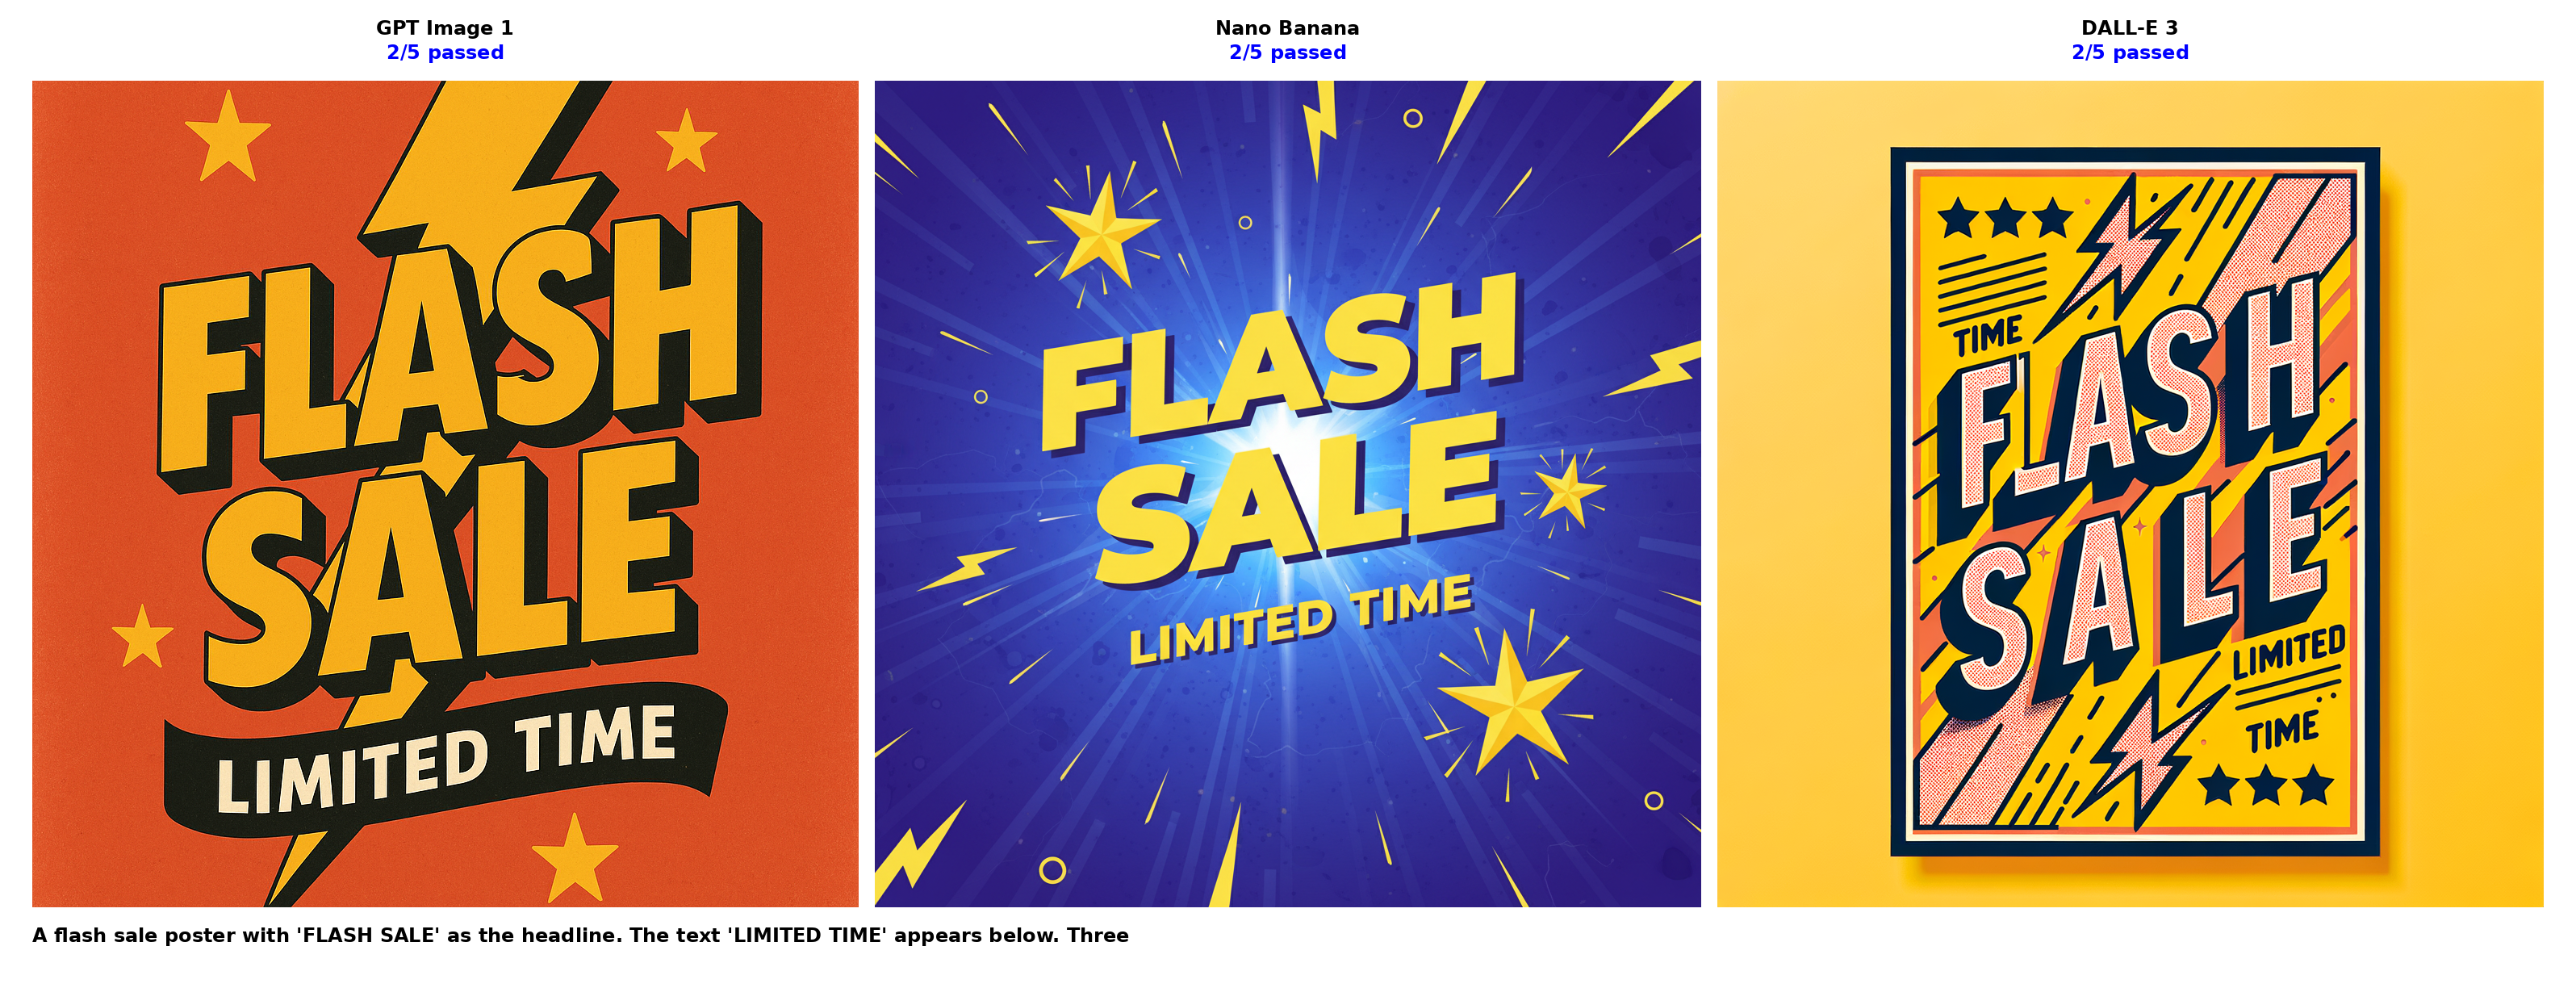
\includegraphics[width=0.95\textwidth]{paper_assets/case_studies/case_study_01_text_005.png}
\caption{Case Study 1: Text Rendering Comparison}
\label{fig:case1}
\end{figure*}

\subsection{Case Study 2: Complex Composition}
\textit{Prompt}: ``A photo of three blue mugs and two red plates on a wooden table. One of the blue mugs is tipped over. The largest blue mug is on the left side of the table, and the smallest red plate is on the right side.'' \textit{Constraints}: Count: 3 mugs, 2 plates; Attribute: Blue mugs, red plates; State: One mug tipped over; Spatial: Largest mug left, smallest plate right. \textit{Results}: GPT Image 1: 2/6 constraints passed (spatial relationships correct). Nano Banana: 2/6 constraints passed. \textit{Analysis}: Models successfully handle spatial relationships but struggle with precise counting and attribute verification.

\begin{figure*}[!t]
\centering
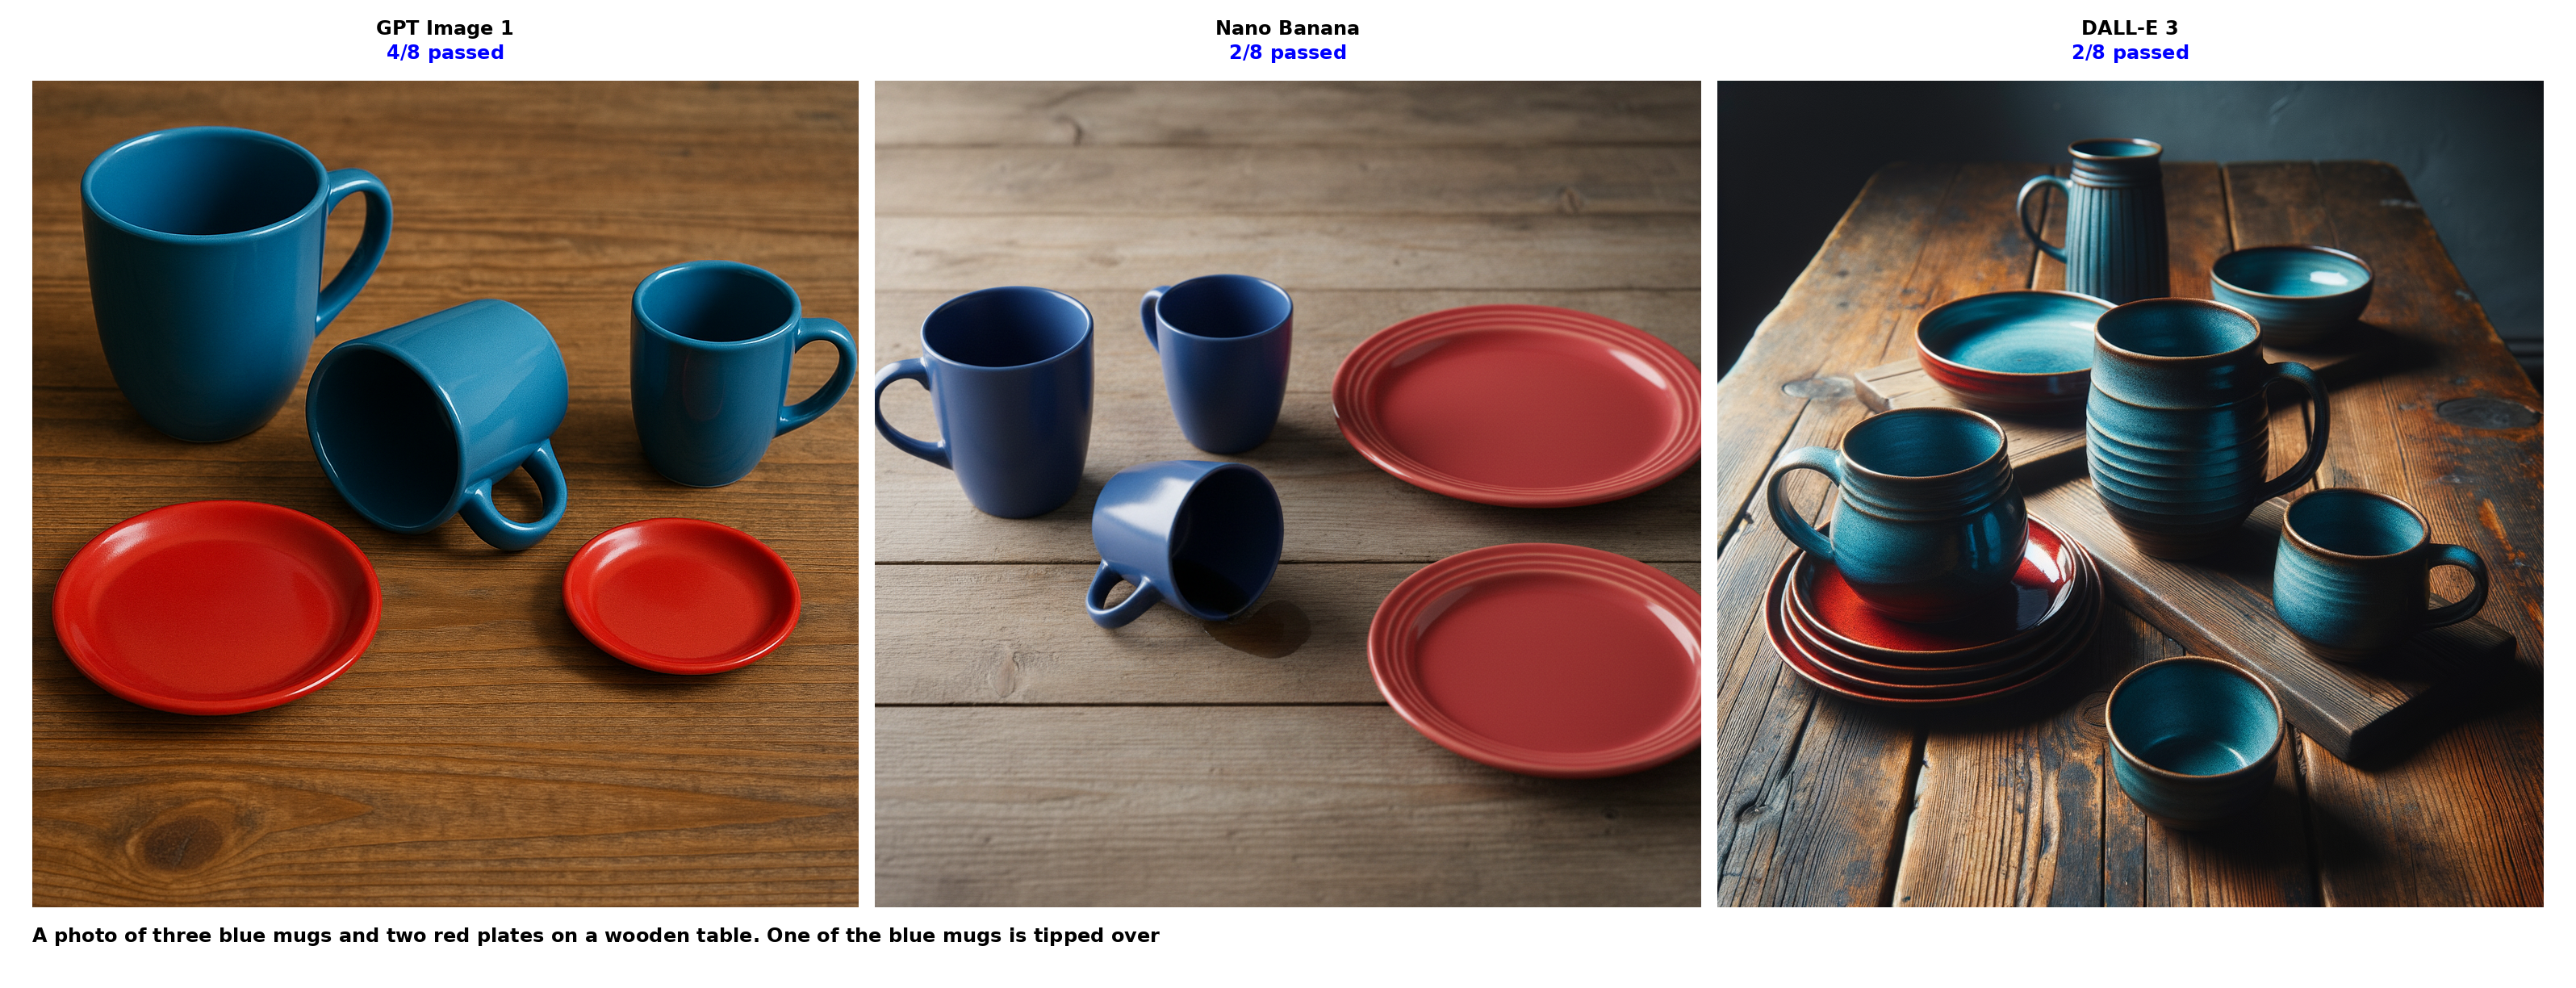
\includegraphics[width=0.95\textwidth]{paper_assets/case_studies/case_study_02_comp_001.png}
\caption{Case Study 2: Complex Composition Comparison}
\label{fig:case2}
\end{figure*}

\subsection{Case Study 3: CSP Constraint}
\textit{Prompt}: CSP task with numeric relationships. \textit{Results}: GPT Image 1: Passed (100\%). Nano Banana: Passed (95\%). \textit{Analysis}: Strong performance on mathematical constraints demonstrates effective OCR and numeric parsing capabilities.

\begin{figure*}[!t]
\centering
\includegraphics[width=0.95\textwidth]{paper_assets/case_studies/case_study_03_csp_01_numbers_row.png}
\caption{Case Study 3: CSP Constraint Comparison}
\label{fig:case3}
\end{figure*}

\section{Cost and Latency Analysis}

\subsection{API Costs}
Estimated costs for the evaluation (based on current API pricing) are shown in Table~\ref{tab:costs}. Note: Costs are estimates based on published API pricing. Actual costs may vary.

\begin{table}[!t]
\renewcommand{\arraystretch}{1.3}
\caption{API Cost Analysis}
\label{tab:costs}
\centering
\begin{tabular}{lccc}
\toprule
Model & Images & Cost/Image & Total Cost \\
\midrule
GPT Image 1 & 47 & \$0.040 & \$1.88 \\
Nano Banana & 47 & \$0.005 & \$0.24 \\
DALL-E 3 & 11 & \$0.040 & \$0.44 \\
\bottomrule
\end{tabular}
\end{table}

\subsection{Cost-Performance Analysis}
Based on estimated costs and performance: \textit{Most Cost-Effective}: Nano Banana (\$0.24 for 47 images, 54.7\% pass rate). \textit{Best Performance}: GPT Image 1 (\$1.88 for 47 images, 58.1\% pass rate). \textit{Cost per Passed Constraint}: GPT Image 1: ~\$0.019 per passed constraint; Nano Banana: ~\$0.003 per passed constraint.

\subsection{Latency}
Latency measurements were not systematically tracked in this evaluation. Future work should include time-to-first-image (TTFI) measurements, end-to-end generation time, API response time analysis, and comparison of synchronous vs. asynchronous generation.

\section{Limitations and Future Work}

\subsection{Current Limitations}
(1) \textit{Incomplete DALL-E 3 Evaluation}: API billing limits prevented full evaluation. (2) \textit{Limited Human Evaluation}: Primarily automated metrics; human preference scores not included. (3) \textit{Cost/Latency Metrics}: Not systematically tracked in current evaluation. (4) \textit{In-Painting Evaluation}: Not included in current benchmark (future addition).

\subsection{Future Directions}
(1) Expand dataset: Add more prompts, especially for in-painting and out-painting tasks. (2) Human evaluation: Incorporate human preference scores and compositional accuracy ratings. (3) Cost analysis: Systematic tracking of API costs and generation latency. (4) Tool usage analysis: Evaluate model selection of generation vs. editing tools. (5) Trajectory visualization: Analyze multi-step generation processes. (6) Additional models: Evaluate Midjourney, Stable Diffusion 3, and other models.

\section{Conclusion}

The Visual Instruction Following Evaluation Benchmark (VIF-Eval) provides a comprehensive framework for assessing generative visual models beyond simple prompt adherence. Our evaluation of three state-of-the-art models reveals: (1) \textit{Strengths}: Models excel at spatial relationships, character consistency, and constraint satisfaction problems; (2) \textit{Weaknesses}: Critical limitations in text rendering (12--13\% pass rate) and precise counting (17--31\% pass rate); and (3) \textit{Comparability}: GPT Image 1 and Nano Banana show similar overall performance (54--58\% pass rates).

The benchmark establishes a foundation for systematic evaluation of visual instruction following capabilities and provides actionable insights for model improvement. Future work should expand the dataset, incorporate human evaluation, and track cost/latency metrics to provide a complete assessment framework.

\begin{thebibliography}{00}
\bibitem{b1} A. Radford et al., ``Learning Transferable Visual Models From Natural Language Supervision,'' in \textit{Proc. ICML}, 2021.
\bibitem{b2} A. Ramesh et al., ``Hierarchical Text-Conditional Image Generation with CLIP Latents,'' in \textit{Proc. NeurIPS}, 2022.
\bibitem{b3} J. Betker et al., ``Improving Image Generation with Better Captions,'' OpenAI Blog, 2023.
\bibitem{b4} R. Rombach et al., ``High-Resolution Image Synthesis with Latent Diffusion Models,'' in \textit{Proc. CVPR}, 2022.
\bibitem{b5} DeepSeek-OCR. [Online]. Available: https://github.com/deepseek-ai/DeepSeek-OCR
\bibitem{b6} GroundingDINO. [Online]. Available: https://github.com/IDEA-Research/GroundingDINO
\bibitem{b7} InsightFace. [Online]. Available: https://github.com/deepinsight/insightface
\end{thebibliography}

\end{document}

